\let\negmedspace\undefined
\let\negthickspace\undefined
\documentclass[journal]{IEEEtran}
\usepackage[a5paper, margin=10mm, onecolumn]{geometry}
%\usepackage{lmodern} % Ensure lmodern is loaded for pdflatex
\usepackage{tfrupee} % Include tfrupee package

\setlength{\headheight}{1cm} % Set the height of the header box
\setlength{\headsep}{0mm}     % Set the distance between the header box and the top of the text

\usepackage{gvv-book}
\usepackage{gvv}
\usepackage{cite}
\usepackage{amsmath,amssymb,amsfonts,amsthm}
\usepackage{algorithmic}
\usepackage{graphicx}
\usepackage{textcomp}
\usepackage{xcolor}
\usepackage{txfonts}
\usepackage{listings}
\usepackage{enumitem}
\usepackage{mathtools}
\usepackage{physics}
\usepackage{gensymb}
\usepackage{comment}
\usepackage[breaklinks=true]{hyperref}
\usepackage{tkz-euclide} 
\usepackage{listings}
% \usepackage{gvv}                                        
\def\inputGnumericTable{}                                 
\usepackage[latin1]{inputenc}                                
\usepackage{color}                                            
\usepackage{array}                                            
\usepackage{longtable}                                       
\usepackage{calc}                                             
\usepackage{multirow}                                         
\usepackage{hhline}                                           
\usepackage{ifthen}                                           
\usepackage{lscape}
\begin{document}

\bibliographystyle{IEEEtran}
\vspace{3cm}

\title{2.10.47}
\author{EE25BTECH11018 - DARISY SREETEJ}
% \maketitle
% \newpage
% \bigskip
{\let\newpage\relax\maketitle}

\renewcommand{\thefigure}{\theenumi}
\renewcommand{\thetable}{\theenumi}
\setlength{\intextsep}{10pt} % Space between text and floats


\numberwithin{equation}{enumi}
\numberwithin{figure}{enumi}
\renewcommand{\thetable}{\theenumi}


\textbf{Question}:
The value of $a$ so that the volume of parallelopiped formed by $\hat{i} + a\hat{j} + \hat{k}, \hat{j} + a\hat{k} \text{ and } a\hat{i} + \hat{k}$ becomes minimum is
\begin{enumerate}
\begin{multicols}{4}
\item $-3$
\item $3$
\item $\frac{1}{\sqrt{3}}$
\item $\sqrt{3}$
\end{multicols}
\end{enumerate}
\textbf{Solution:}
Let us consider,
\begin{align*}
\vec{p}=\hat{i}+a\hat{j}+\hat{k}\\
\vec{q}=\hat{j}+a\hat{k}\\
\vec{r}=a\hat{i}+\hat{k}
\end{align*}

then, the Volume of the parallelopiped formed by $\vec{p},\vec{q},\vec{r}$ is ,
\begin{align}
    V = \vec{p}\cdot(\vec{q}\times\vec{r})
\end{align}
\begin{align}
V=\mydet{
    1 && a && 1\\
    0 && 1 && a\\
    a && 0 && 1
    }
\end{align}
\begin{align}
    V=a^3-a+1
\end{align}
Now , consider
\begin{align}
    f(a)=a^3-a+1\\
    f'(a)=3a^2+1
\end{align}
\begin{align*}
\text{Set }f'(a)=0  \Rightarrow a^2=\frac{1}{\sqrt{3}} \Rightarrow a=\frac{1}{\sqrt{3}} or -\frac{1}{\sqrt{3}} 
\end{align*}
\begin{align}
\text{Second derivative }f''(a)=6a\\
\text{At }a=\frac{1}{\sqrt{3}},f''>0 \Rightarrow minimum\\
\text{At }a=-\frac{1}{\sqrt{3}},f''<0 \Rightarrow maximum
\end{align}
Therefore , $a=\frac{1}{\sqrt{3}}$ for which the Volume of the parallelopiped becomes minimum.
\begin{figure}[h!]
  \centering
  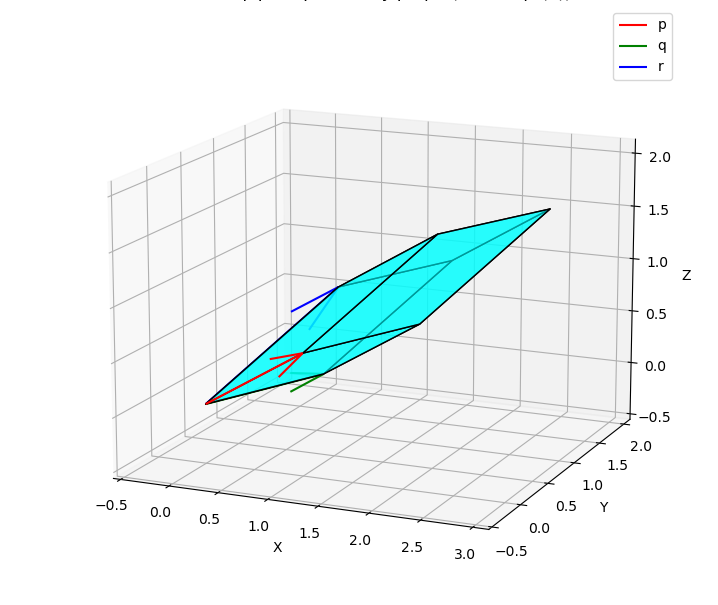
\includegraphics[width=0.7\columnwidth]{figs/fig.png} 
   \caption*{Parallelopiped with Vectors $\vec{p},\vec{q},\vec{r}$ for which $a=\frac{1}{\sqrt{3}}$(Volume is minimum)}
  \label{Fig1}
\end{figure}



\end{document}